\documentclass{beamer}
\usepackage{beamerthemeshadow}
\usepackage{verbatim}

\usepackage{lastpage}
\usepackage{xcolor}
\usepackage{pgf}
\usepackage{colortbl}
\usepackage{hyperref}
\usepackage{multirow}
\usepackage{dsfont}
\usepackage{graphbox}


\usepackage{siunitx}
\sisetup{input-symbols=(), group-digits  = false} 

\newcommand{\bi}{\begin{itemize}}
\newcommand{\ei}{\end{itemize}}
\newcommand{\be}{\begin{enumerate}}
\newcommand{\ee}{\end{enumerate}}
\newcommand{\bd}{\begin{description}}
\newcommand{\ed}{\end{description}}
\newcommand{\prbf}[1]{\textbf{#1}}
\newcommand{\prit}[1]{\textit{#1}}
\newcommand{\beq}{\begin{equation}}
\newcommand{\eeq}{\end{equation}}
\newcommand{\bdm}{\begin{displaymath}}
\newcommand{\edm}{\end{displaymath}}

\newcommand{\ft}[1]{
  \frametitle{\begin{tabular}{p{4.2in}r} \textcolor{white}{#1} & \small{\insertframenumber / \inserttotalframenumber} \end{tabular}}
  \setbeamercovered{transparent=18}
}

\newcommand{\eft}[1]{
  \frametitle{\begin{tabular}{p{4in}r} \textcolor{white}{#1} & \small{\hyperlink{f:questions}{\beamergotobutton{GO BACK}}} \end{tabular}}
  \setbeamercovered{transparent=18}
}

\newcommand{\stepinv}{\setbeamercovered{invisible}}
\newcommand{\stopinv}{\setbeamercovered{transparent=18}}
\newcommand{\uncoverinv}[1]
{
  \setbeamercovered{invisible}
  \uncover<+->{#1}
  \setbeamercovered{transparent=18}
}
\newcommand{\ans}[1]{\textcolor{blue}{#1}}
\newcommand{\ansinv}[1]
{
  \setbeamercovered{invisible}
  \uncover<+->{\textcolor{blue}{#1}}
  \setbeamercovered{transparent=18}
}
\newcommand{\setinv}{\setbeamercovered{invisible}}
\newcommand{\setvis}{\setbeamercovered{transparent=18}}
\newcommand{\centerpic}[2]
{
  \begin{center}
  \includegraphics[#1]{#2}
  \end{center}
}
\newcommand{\h}[1]{\hat{#1}}
\newcommand{\ds}{\displaystyle}

\definecolor{light}{rgb}{1.0,0.7,0.7}
\definecolor{BrickRed}{rgb}{0.8,0.1,0.1}
%\definecolor{light}{rgb}{1.0,0.5,0.5}
\newcommand{\hl}[1]{\only<#1>{\cellcolor{light}}}

\definecolor{mycolor}{rgb}{0.25,0.0,0.37}
\usecolortheme[named=mycolor]{structure}

\title[Regime Switching in Fiscal Debt \& Composition]{Regime Switching in Fiscal Debt Targets and Fiscal Composition}
\author[Dr. James M. Murray, University of Wisconsin - La Crosse]
{
James M. Murray, Ph.D.\\
Department of Economics\\
University of Wisconsin - La Crosse
}
\date{April 10, 2017}

\begin{document}

\frame{\titlepage \setcounter{framenumber}{0}}

\begin{frame}
  \ft{Purpose}
  \uncover<+-> {
  \begin{block}{Describe fiscal policy dynamics}
    \begin{tabular}{ll}
    Government expenditures & Deficits \\
    Income tax rate & Debt \\
    Net transfer payments
    \end{tabular}
  \end{block}
  } % end uncover

  \uncover<+->{
  \begin{block}{Describe debt service}
    \begin{enumerate}
    \item How do these fiscal policy variables respond to \textit{debt / GDP}?
    \item What is the implied target for \textit{debt / GDP}?
    \item Is there switching in these fiscal policy responses?
    \item Is there switching in the long-run debt target?
    \end{enumerate}
  \end{block}
  } % end uncover

  \uncover<+->{
  \begin{block}{Describe stabilizing behavior}
    \begin{enumerate}
    \item How do fiscal policy variables respond to \textit{output gap}?
    \item Is there switching in these fiscal policy responses?
    \end{enumerate}
  \end{block}
  } % end uncover
\end{frame}

\begin{frame}
  \ft{Fiscal Variables}
  \begin{tabular}{cp{1.5in}}
    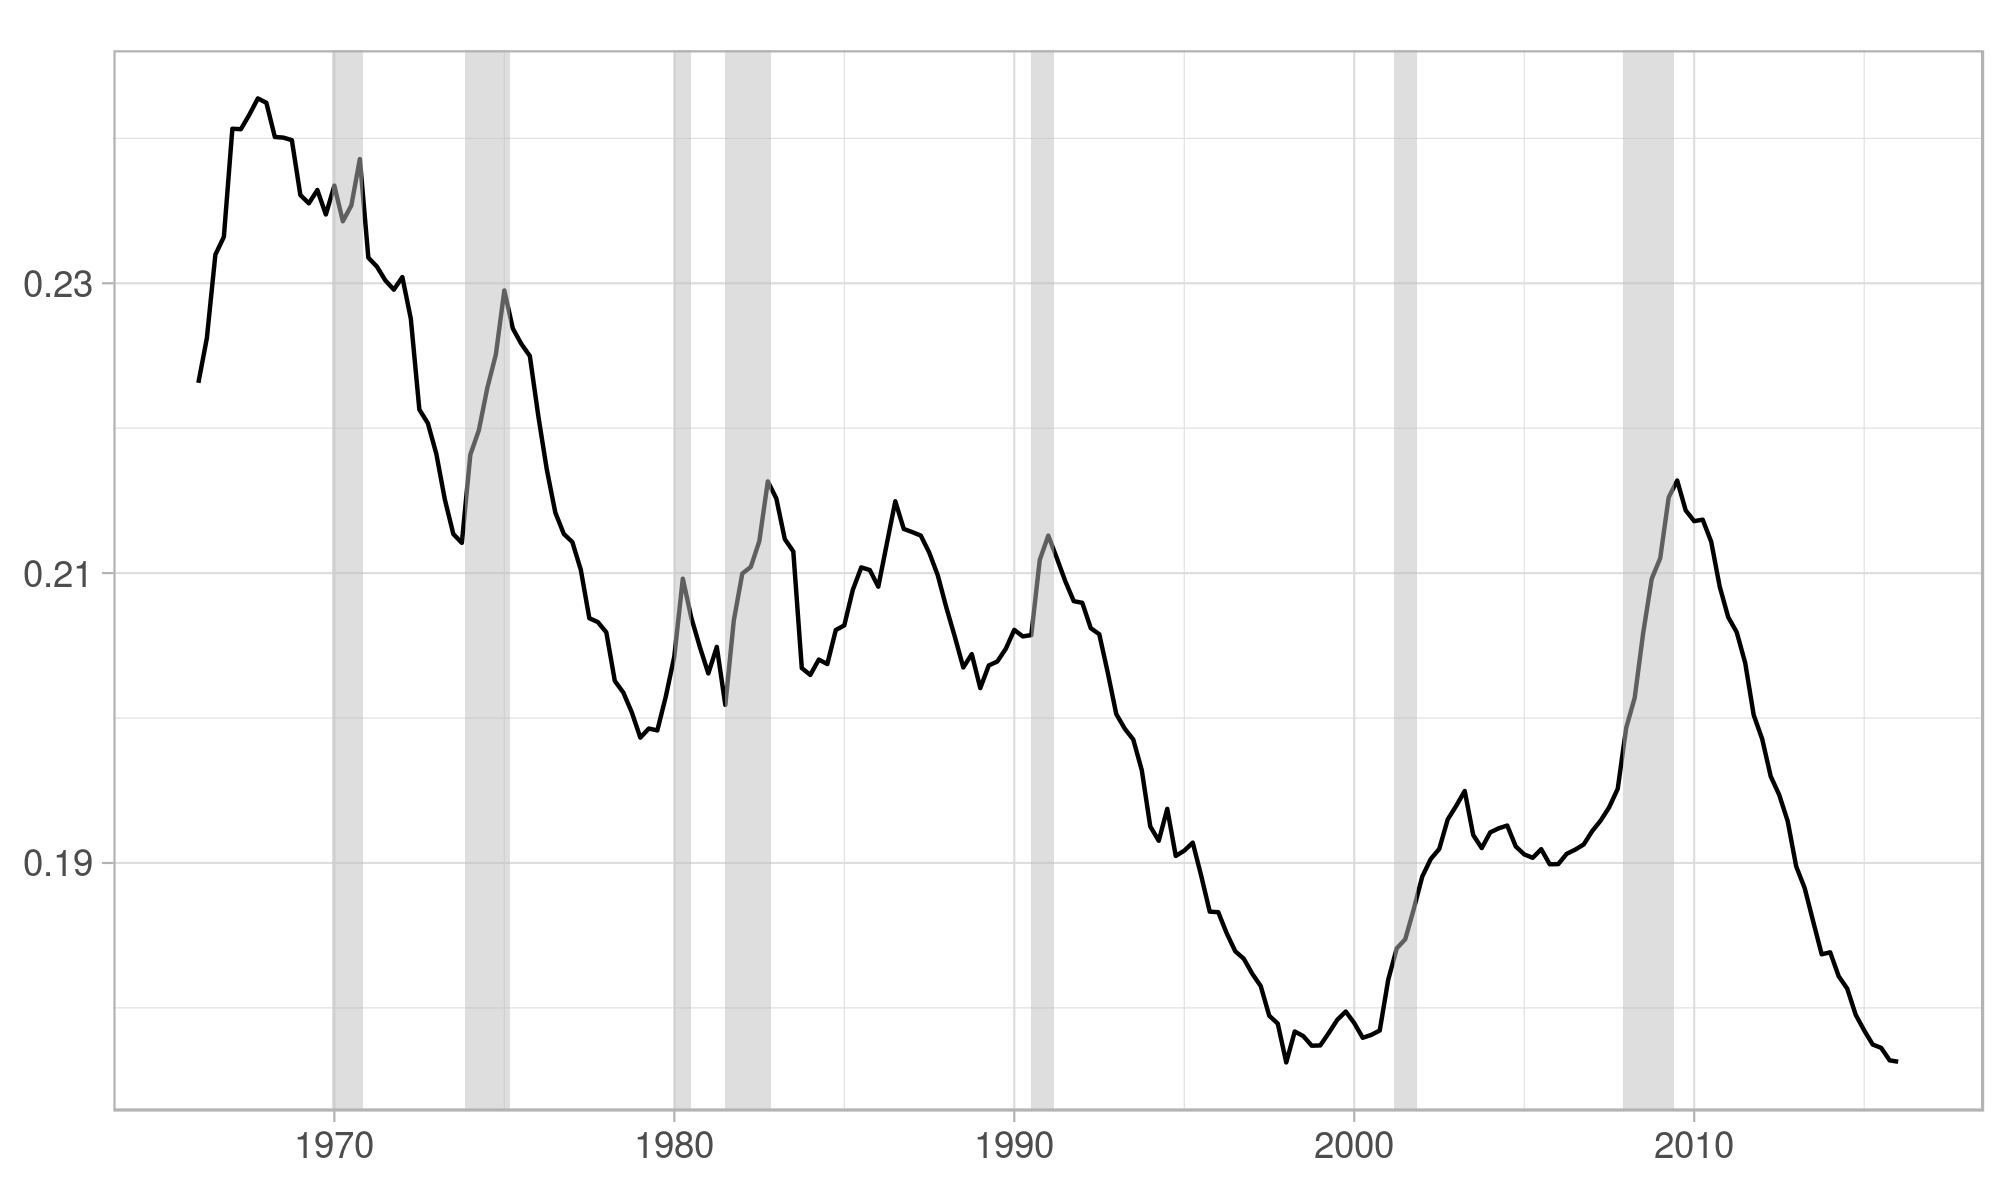
\includegraphics[align=t,height=0.41\textheight]{./gov.png} & \vspace*{2pc}Government Spending / GDP Ratio \\
    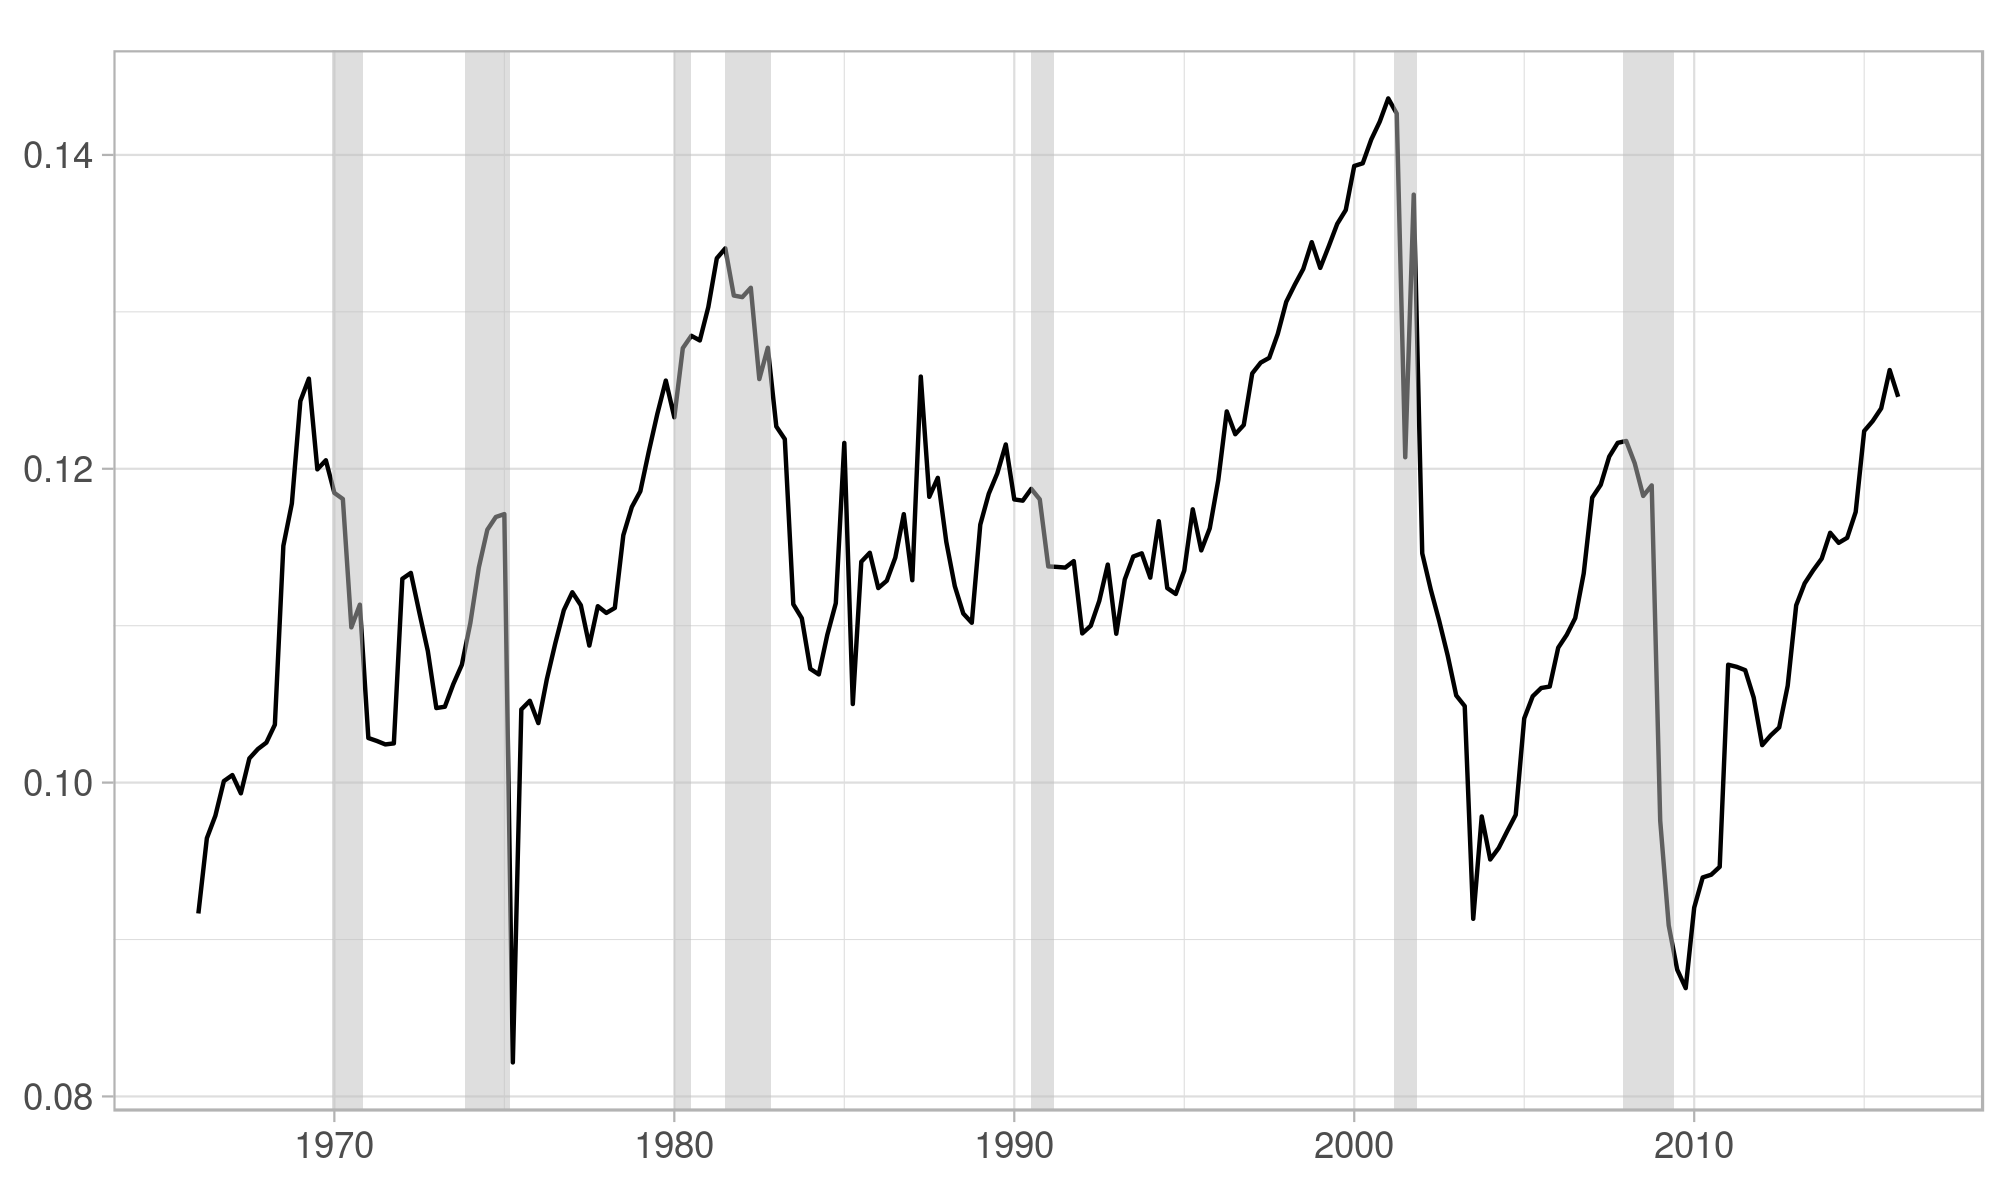
\includegraphics[align=t,height=0.41\textheight]{./tax.png} & \vspace*{2pc}Federal Tax Revenue / GDP Ratio \\
  \end{tabular}
\end{frame}

\begin{frame}
  \ft{Fiscal Variables}
  \begin{tabular}{cp{1.5in}}
    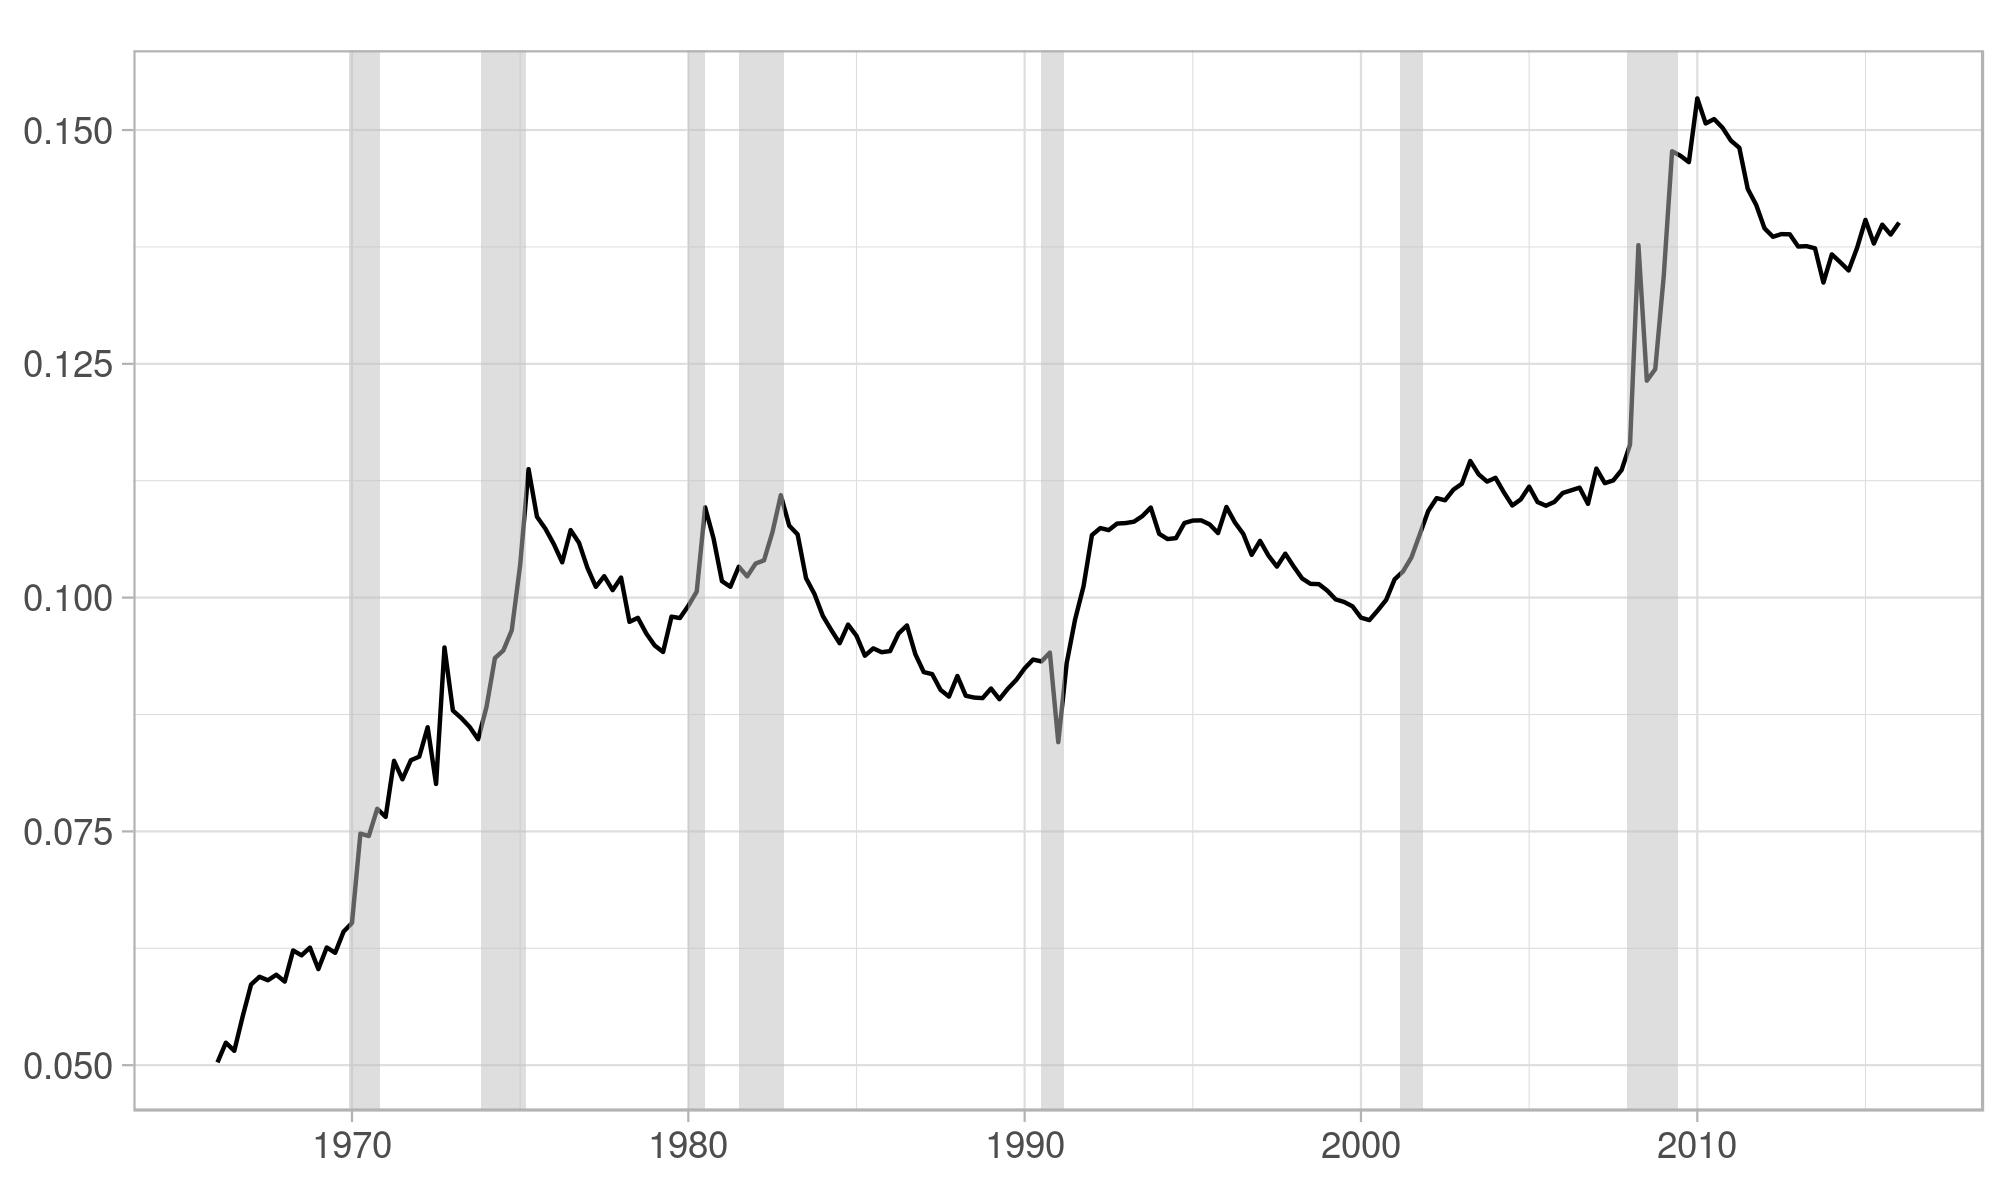
\includegraphics[align=t,height=0.41\textheight]{./transfers.png} & \vspace*{2pc}Transfers / GDP Ratio \\
    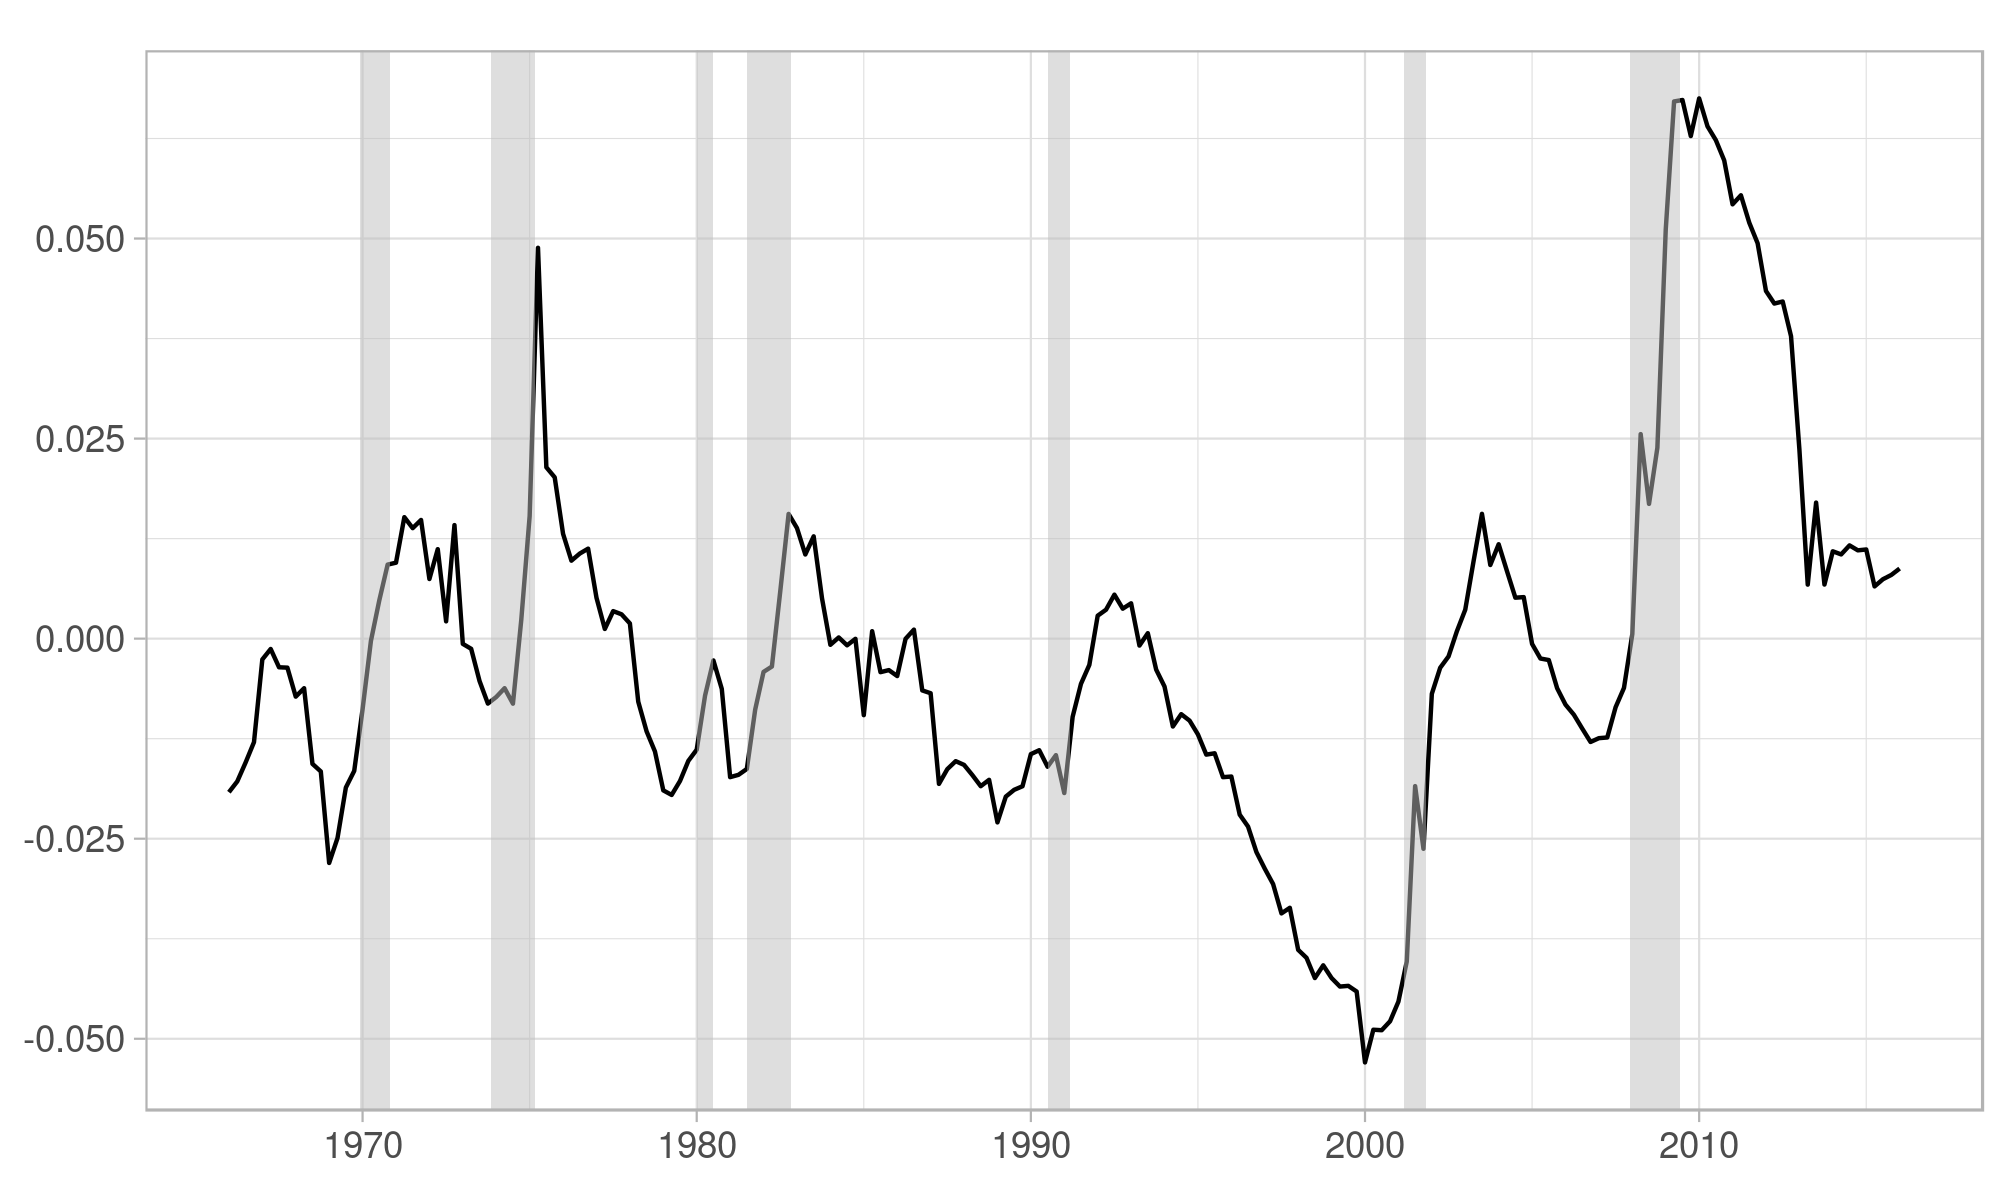
\includegraphics[align=t,height=0.41\textheight]{./deficit.png} & \vspace*{2pc}Deficit / GDP Ratio \\
  \end{tabular}
\end{frame}

\begin{frame}
  \ft{Fiscal Variables}
  \begin{tabular}{cp{1.5in}}
    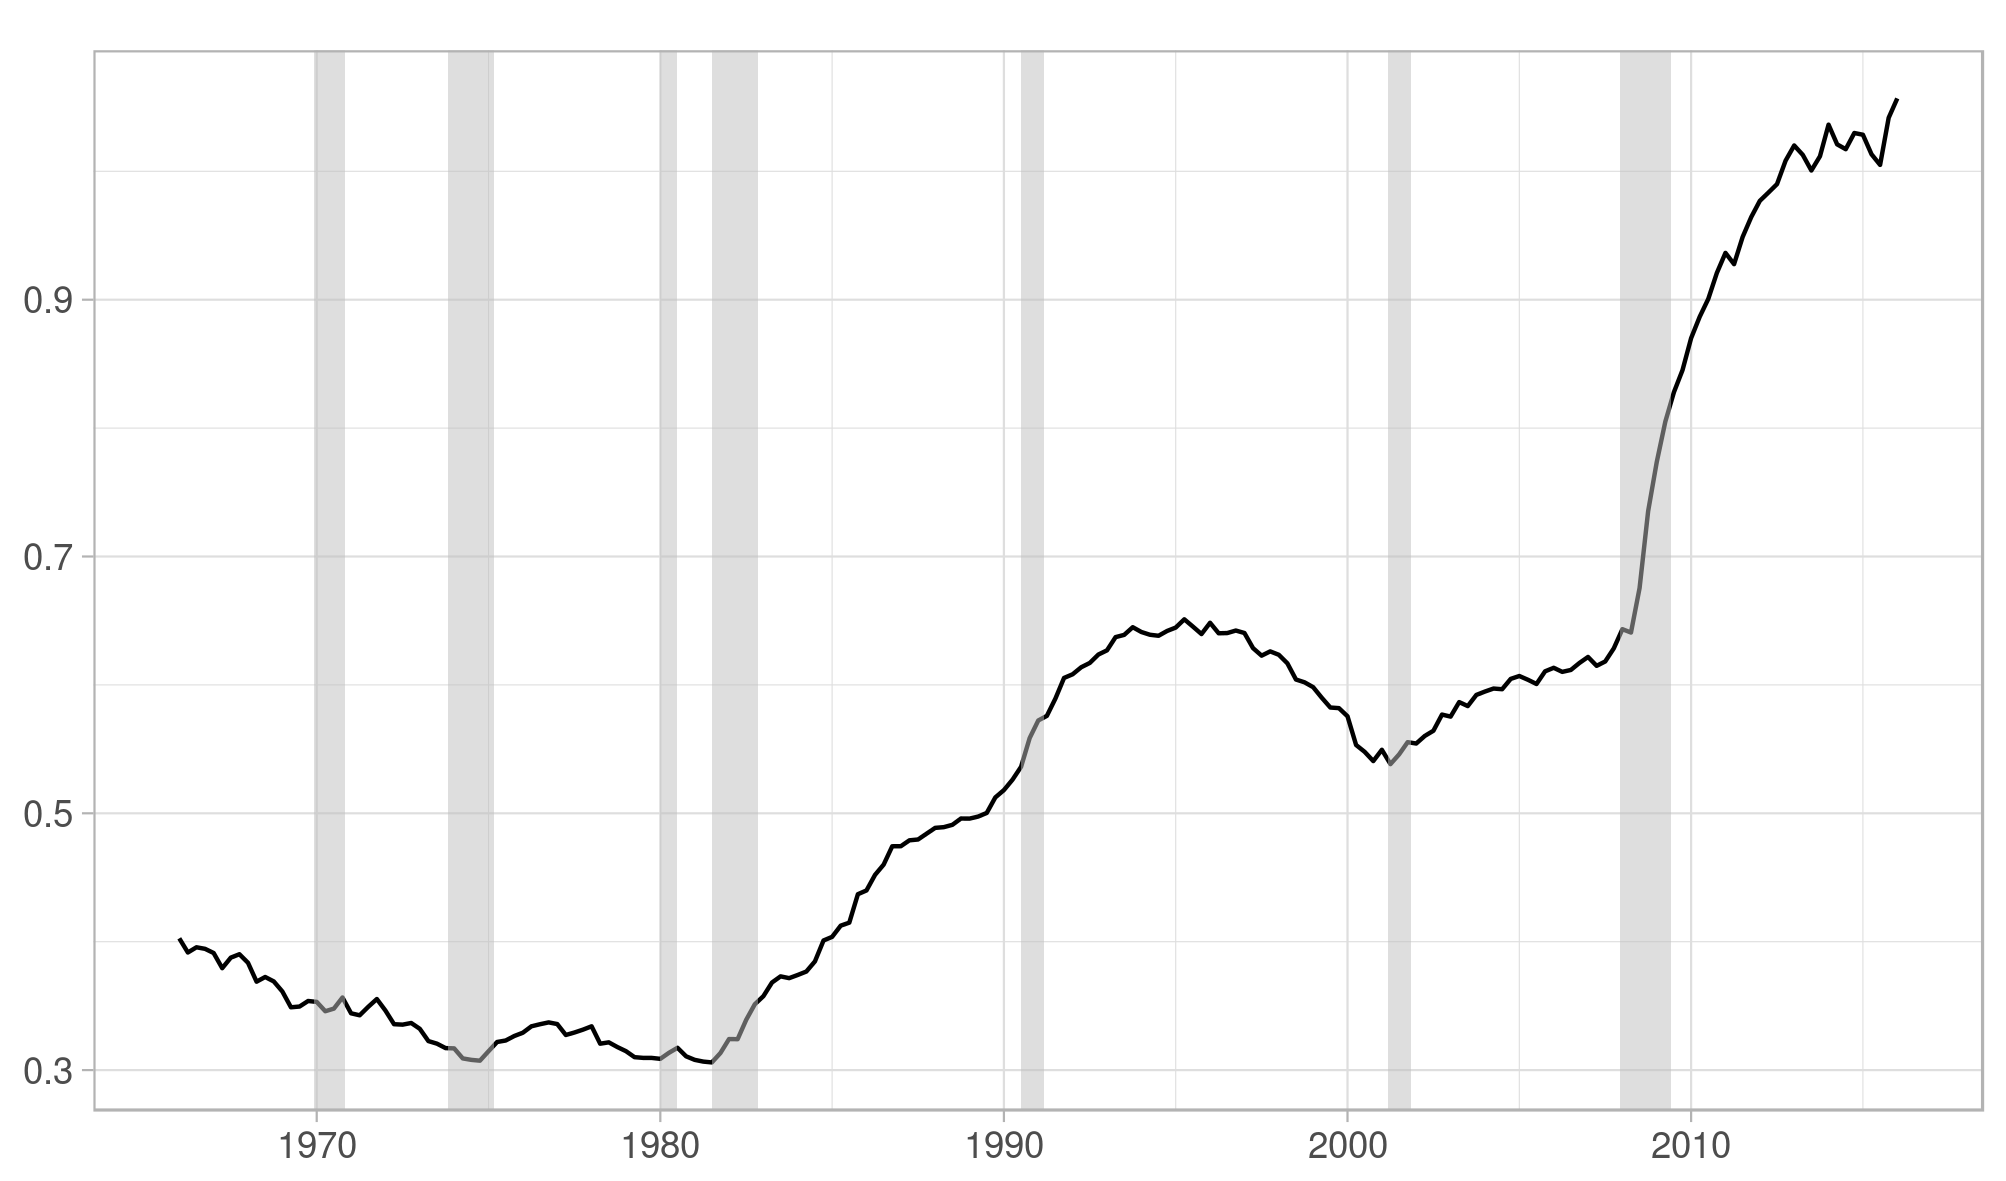
\includegraphics[align=t,height=0.41\textheight]{./debt.png} & \vspace*{2pc}Debt / GDP Ratio \\
  \end{tabular}
\end{frame}

\begin{frame}
  \ft{Fiscal dynamics matter}
  \uncover<+-> {
    \begin{block}{Debt target and tax response matter}
      \bi
      \item Expected smaller debt/GDP target and/or expected larger response of taxes to debt,\newline
        $\rightarrow$ Higher expected income taxes\newline
        $\rightarrow$ lower consumption, investment, real GDP.
      \item Richter and Throckmorton (EER, 2015):
        \bi
        \item Unknown debt targets amplify impact of tax shocks
        \item Uncertain long-run debt targets reduced impact of ARRA, extensions to Bush tax cut
        \ei
    \end{itemize}
  \end{block}
  } % end uncover

  \uncover<+-> {
  \begin{block}{Fiscal composition matters}
    Leeper, Plante, and Traum (JoE, 2010)
    \begin{itemize}
    \item Rich set of fiscal variables responding to debt fits data best
    \item Magnitude of fiscal shocks depend on composition
    \item Fiscal multipliers can have unexpected signs, depending on composition
    \end{itemize}
  \end{block}
  } % end uncover
\end{frame}

\begin{frame}
  \ft{Related fiscal policy literature}
    \uncover<+->{
    \begin{block}{Fiscal policy switching}
      \begin{itemize}
      \item Favero and Montecelli (2005): Deficit feedback rule with \textit{Markov~switching}
        \begin{itemize}
        \item Switching explains data better
        \item Deficits switch between \textit{active} and \textit{passive} regimes
        \end{itemize}
      \item Ko and Morita (2013): Switching in government expenditures and taxes in Japan    
      \end{itemize}
    \end{block}
    }

    \uncover<+->{
    \begin{block}{Switching and Monetary/Fiscal Interactions}
      \begin{itemize}
      \item Eg: Chung, Davig, Leeper (2007), Davig and Leeper (2011)
      \item Evidence for switching between active/passive fiscal and monetary policies
      \item Implications for fiscal multipliers and stabilizing impact of monetary policy
      \end{itemize}
    \end{block}
    }
\end{frame}

\begin{frame}
  \ft{Fiscal Policy: Government Expenditures}
  \uncover<+->{\begin{block}{Gradual movement toward target} 
  \bdm G_t = \rho_g G_{t-1} + \left(1-\rho_g\right) G_t^*, \edm
  \vspace*{-1pc}\begin{itemize}
    \item $\rho_g \in (0,1)$ persistence parameter
    \item $G_t$: Actual nominal government expenditures
    \item $G_t^*$: Target level for government expenditures
  \end{itemize}
  \end{block}}
 
  \uncover<+->{\begin{block}{Divide by nominal GDP ($Y_t$)}
  \bdm g_t = \rho_g \left( \frac{1}{y_t} \right) g_{t-1} + \left(1-\rho_g\right) g_t^* \edm
  \begin{itemize}
    \item $g_t \equiv G_t/Y_t$, $g_t^* \equiv G_t^*/Y_t$: Actual / Target government expenditures to GDP ratio
    \item $y_t \equiv Y_t/Y_{t-1}$: Gross growth rate of nominal GDP
  \end{itemize}
  \end{block}}
\end{frame}

\begin{frame}
  \ft{Fiscal Policy: Government Expenditures Target}

  \uncover<+->{
  \begin{block}{Target Policy Behavior}
    \begin{itemize}
    \item Use government expenditures to stabilize business cycle\\
      $\rightarrow$ Decrease gov exp in response to output gap 
    \item Decrease government expenditures in response to rising debt
    \item Long-run target for government expenditures / GDP ratio
    \end{itemize}
  \end{block}
  }

  \uncover<+->{
  \begin{block}{Structure}
    \bdm g_t^* = \bar{g}(s_t) + \psi_g(s_t) x_t + \gamma_g(s_t) \left[ b_{t-1} - \bar{b}(s_t) \right] + u_{g,t}, \edm
    \vspace*{-1.5pc}\begin{itemize}
    \item $s_t \in \{1,..,M\}$: Fiscal regime... more later
    \item $\bar{g}(s_t)$: Long-run government expenditures / GDP target
    \item $b_{t-1}$: Lagged government debt / GDP ratio
    \item $\bar{b}(s_t)$ Long-run target debt / GDP ratio
    \item $\psi_g(s_t) < 0$: Response to increase in output gap
    \item $\gamma_g(s_t)<0$: Response to increase in government debt
    \end{itemize}
  \end{block}
  }
\end{frame}


\begin{frame}
  \ft{Fiscal Policy Behavior}

  \begin{block}{Fiscal policy variables}
    \bdm f_t \in \left\{ \begin{array}{ll}
      g_t: \mbox{ Gov exp / GDP}, & n_t: \mbox{ Net transfers / GDP} \\
      \tau_t: \mbox{ Taxes / GDP}, & d_t: \mbox{ Deficits / GDP} \\
    \end{array} \right\} \edm
    \vspace*{-1pc}
  \end{block} 

  \begin{block}{Similar evolution for all fiscal variables}
    \bdm f^*_t = \bar{f}(s_t) + \psi_f(s_t) x_t + \gamma_f(s_t) \left[ b_{t-1} - \bar{b}(s_t) \right] + u_{f,t},\edm
    \bdm u_{f,t} = \alpha_f u_{f,t-1} + \epsilon_{f,t},~\epsilon_{f,t}\sim \mathcal{N}\left(0, \sigma_f^2(s_t)\right) \edm
  \end{block}

  \begin{block}{Notation}
    \begin{scriptsize}
    \begin{tabular}{llcll}
      $f_t$ & Fiscal variable &  & $x_t$ & Output gap \\ 
      $f_t^*$ & Time $t$ target for $f_t$ & & $\rho_f$ & Persistence of $f_t$ \\
      $\bar{f}(s_t)$ & \textit{Long-run} target for $f_t$ & & $\psi_f(s_t)$ & Feedback on output gap \\
      $b_t$ & Debt / GDP ratio & & $\gamma_f(s_t)$ & Feedback on debt/GDP \\
      $\bar{b}(s_t)$ & \textit{Long-run} target for debt/GDP & & $u_{f,t}$ & Innovations to $f_t$ \\
    \end{tabular}
    \end{scriptsize}
  \end{block}
  
\end{frame}


\begin{frame}
  \ft{Government Budget Constraint}
  \begin{small}
  \uncover<+->{
  \begin{block}{Intertemporal government budget constraint}
  \bdm B_t = (1 + r_{t-1}) B_{t-1} + D_t - \left( M_t - M_{t-1} \right), \edm
  \begin{tabular}{ll}
    $B_t$: Nominal government debt & $r_{t-1}$: interest rate on past-issued debt \\
    $D_t$: Nominal budget deficit & $M_t - M_{t-1}$: seigniorage
  \end{tabular}
  \end{block}
  }

  \uncover<+->{
  \begin{block}{Empirical government budget constraint}
    Divide both sides by $Y_t$ and allow for measurement error ($v_t$)
    \only<1-2>{\bdm b_t = (1+r_{t-1}) \left(\frac{1}{y_t}\right) b_{t-1} + d_t - m_t + \left(\frac{1}{y_t}\right) m_{t-1} + v_t \edm
      \vspace*{5pc} }
    \only<3->{\bdm b_t = (1+r_{t-1}) \left(\frac{1}{y_t}\right) b_{t-1} + d_t \textcolor{red}{\underbrace{\displaystyle~ -~ m_t + \left(\frac{1}{y_t}\right) m_{t-1} + v_t}_{\mbox{Residual: } \displaystyle u_{b,t}}} \edm
    }
    \only<3>{\vspace*{3.55pc}}
    \only<4->{
    \bdm b_t = (1+r_{t-1}) \left(\frac{1}{y_t}\right) b_{t-1} + d_t + u_{b,t} \edm
    \bdm u_{b,t} = (1-\alpha_b) \bar{u}_b + \alpha_b u_{b,t-1} + e_{b,t} \edm
    }
  \end{block}
  }
  \end{small}
\end{frame}

\begin{frame}
  \ft{Relationship between deficits and debt}
  \uncover<+->{\begin{block}{Budget constraint}
  \bi
\item Budget constraint describes relationship between long-run targets for...\\
  $~~$(1) Debt / GDP, $\bar{b}(s_t)$, and\\
  $~~$(2) deficits / GDP, $\bar{d}(s_t)$
  \item Evaluate budget constraint at steady state and a constant fiscal regime $s_{t-1}=s_t=s$:
    \bdm \bar{d}(s) = \left( \frac{\bar{y}-\bar{r}-1}{\bar{y}} \right) \bar{b}(s) - \bar{u}_b \edm
    \ei
  \end{block}}

  \uncover<+->{
  \begin{block}{Long-run deficit dependencies}
    \begin{tabular}{ll}
    Debt target & Long-run nominal interest rate \\
    Long-run nominal GDP growth & Long-run seigniorage 
    \end{tabular}
    
    \ \\
    Jointly estimate these long-run targets 
  \end{block}}  
\end{frame}

\begin{frame}
  \ft{Variances}
  \uncover<+->{
  \begin{block}{Regime-dependent variances for fiscal shocks}
    \begin{tabular}{ll}
      $\sigma_g^2(s_t)$: Var(shock to gov exp) & $\sigma_n^2$: Var(shock to transfers) \\
      $\sigma_\tau(s_t)$: Var(shock to taxes) & $\sigma_d^2$: Var(shock to deficits) \end{tabular}
  \end{block}}

  \uncover<+->{
  \begin{block}{Correlations of fiscal shocks}
    \begin{itemize}
    \item Fiscal policy decisions are dependent on one another.
    \item Consider all possible correlations:\\
      \hspace{2pc} $\varrho_{g,\tau}$, $\varrho_{\tau,n}$, $\varrho_{g,n}$, $\varrho_{\tau,d}$, $\varrho_{g,d}$, $\varrho_{n,d}$
    \end{itemize}
  \end{block}
  }
\end{frame}

\begin{frame}
  \ft{Three Sources for Regime Switching}
  \begin{footnotesize}
  \uncover<+->{\begin{block}{Long-run Debt Target Regimes}
    \begin{enumerate}[{Regime} A:]
      \setcounter{enumi}{11}
      \item \textit{Low} long-run target for debt/GDP (low value for  $\bar{b}(s_t)$)
      \setcounter{enumi}{7}
      \item \textit{High} long-run target for debt/GDP (high value for  $\bar{b}(s_t)$)
    \end{enumerate}
  \end{block}}

  \uncover<+->{
    \begin{block}{Fiscal Financing}
      \bi
      \item Targets for fiscal components: $\bar{g}(s_t)$, $\bar{\tau}(s_t)$, $\bar{n}(s_t)$, $\bar{d}(s_t)$
      \item Behavior toward output gap and debt: $\psi_f(s_t)$ and $\gamma_f(s_t)$, for $f \in \{g,\tau,n,d\}$
      \ei
        
      \vspace*{-0.5pc}\begin{enumerate}[{Regime} 1:]
      \item Fiscal behavior 1
      \item Fiscal behavior 2
      \end{enumerate}
    \end{block}
  }

  \uncover<+->{
    \begin{block}{Fiscal Volatility}
      Two regimes to determine variances, $\sigma_g^2(s_t)$, $\sigma_\tau^2(s_t)$, $\sigma_n^2(s_t)$, and $\sigma_d^2(s_t)$:
      \begin{enumerate}[{Regime} A:]
        \setcounter{enumi}{18}
        \item \textit{Stable}, relatively smaller variances
        \setcounter{enumi}{21}
        \item \textit{Volatile}, relatively larger variances 
      \end{enumerate}
    \end{block}
  }
  \end{footnotesize}
  
\end{frame}


\begin{frame}
  \ft{Possible Regimes}
  \begin{footnotesize}
  \uncover<+->{\begin{block}{Eight regime combinations are possible!}
    \begin{tabular}{lll}
      (L) Low debt, & (1) Financing Regime 1, & (S) Low volatility$~~$ \\ (H) High debt, & (1) Financing Regime 1, & (S) Low volatility    \\
      (L) Low debt, & (2) Financing Regime 2, & (S) Low volatility$~~$ \\ (H) High debt, & (2) Financing Regime 2, & (S) Low volatility    \\
      (L) Low debt, & (1) Financing Regime 1, & (V) High volatility$~~$ \\  (H) High debt, & (1) Financing Regime 1, & (V) High volatility    \\
      (L) Low debt, & (2) Financing Regime 2, & (V) High volatility$~~$ \\  (H) High debt, & (2) Financing Regime 2, & (V) High volatility
    \end{tabular}
  \end{block}}

  \uncover<+->{\begin{block}{Regime matters. Suppose taxes increased.  Was this..}
    \bi
    \item<+-> one time shock, no change in regime?
    \item<+-> change in long-run target for debt/GDP?
    \item<+-> change in long-run target for taxes/GDP?
    \item<+-> change in policy using taxes more heavily to repay debt
    \item<+-> change in policy where taxes are more/less response to output gap
    \item<+-> one time shock, but evidence of more volatile policy shocks to come
    \ei
  \end{block}}
  \end{footnotesize}
\end{frame}


\begin{frame}
  \ft{Estimation Goals}
  
  \uncover<+->{\begin{block}{Describe Regimes}
    \bi
    \item How large is debt/GDP ratio in each regime?
    \item Describe how fiscal financing regimes are different.
    \item How large are differences in volatility regimes.
    \ei
  \end{block}}

   \uncover<+->{\begin{block}{Identify Time Periods}
    For each quarter over 1966-2016, identify probabilities that fiscal policy was in each regime.
  \end{block}}
\end{frame}

\begin{frame}
  \ft{Regime Switching Procedure}
  \begin{footnotesize}
  \uncover<+-> {
  \begin{block}{Markov regime switching}
    Action to remain/switch determined randomly
    \vspace*{-0.5pc}
    \bdm P(s_t=1) = p_1 ~\mathds{1}(s_{t-1}=1) + (1-p_2) ~\mathds{1}(s_{t-1}=2) \edm
    \bdm P(s_t=2) = (1-p_1) ~\mathds{1}(s_{t-1}=1) + p_2 ~\mathds{1}(s_{t-1}=2) \edm
    \vspace*{-1.5pc}
    \bi
    \item $p_1=P(s_t=1 | s_{t-1}=1)$ be prob policy remains in reg 1
    \item $p_2=P(s_t=2 | s_{t-1}=2)$ be prob policy remains in reg 2
    \ei
  \end{block}}

  \uncover<+->{\begin{block}{Independent sources of regime switching} 
      \bi
      \item Same \textit{independent} regime switching procedure for each source
      \item Independent regime switching allows for rich possibilities:
      \bi
      \item Changes in priorities for taxes, transfers, spending, \textit{without adjusting long-run targets for debt/GDP}
      \item Changes in debt-targets, \textit{without adjusting purposes and priorities for fiscal components}
      \item Changes in volatility of fiscal outcomes, \textit{without changing goals or purposes}
        \ei
      \ei
  \end{block}}
  \end{footnotesize}
\end{frame}

\begin{frame}
  \ft{Completing the model}
  \uncover<+->{\begin{block}{Loose ends}
  \bi
  \item Relationship between $\bar{d}(s_t)$ and $\bar{b}(s_t)$ depends on...
    \bi
    \item long-run values for nominal GDP growth ($\bar{y}$)
    \item long-run average interest rate ($\bar{r}$)
    \ei  
  \item Identify effects of output gap on fiscal policy behavior \textit{from effects of fiscal policy actions on output gap}.
  \ei
  \end{block}}

  \uncover<+->{\begin{block}{Next steps}
    \bi
    \item Specify monetary policy
    \item Specify inter-dependent behavior of macro variables:\newline GDP growth, output gap, and inflation
    \ei
  \end{block}}
\end{frame}

\begin{frame}
  \ft{Monetary Policy}
  \uncover<+->{\begin{block}{Taylor-like (1993) rule}
  \bdm r_t = (1-\rho_r) \bar{r} + \rho_r r_{t-1} + (1-\rho_r) \left[\phi_x x_t + \phi_\pi \left(\pi_t - \bar{\pi}\right) \right] + u_{r,t}, \edm
  \begin{tabular}{ll}
    $\bar{r}$: long-run nominal interest rate & $\pi_t$: inflation rate \\
    $\rho_r$: Monetary policy persistence & $\bar{\pi}$: target inflation rate \\
    $\phi_x > 0$: Response to output gap & $x_t$: output gap \\
    $\phi_\pi >0$: Response to inflation & $u_{r,t}$: shock to monetary policy \\
  \end{tabular}
  \end{block}}

  \uncover<+->{\begin{block}{Policy shock}
      \bdm u_{r,t} = \alpha_r u_{r,t-1} + e_{r,t}, ~~ e_{r,t} \sim \mathcal{N}\left(0, \sigma_r^2\right) \edm
  \end{block}}
\end{frame}

\begin{frame}
  \ft{Output and Inflation Dynamics}
  \uncover<+->{\begin{block}{Dependent variables}
  Augmented vector autoregression for...
  \be
  \item nominal GDP growth, $y_t$,
  \item output gap, $x_t$, 
  \item inflation, $\pi_t$
  \ee
  \end{block}}

  \uncover<+->{\begin{block}{Explanatory variables}
    \bi
    \item One lag of all dependent variables: $y_{t-1}$, $x_{t-1}$, $\pi_{t-1}$
    \item Fiscal policy variables: $g_t$, $\tau_t$, $n_t$
    \item Monetary policy: $r_t$
      \ei
  \end{block}}

  \uncover<+->{\begin{block}{Estimation Outcomes}
    \bi
    \item Long-run values for $\bar{y}$ and $\bar{r}$
    \item Predictive model for impact of fiscal policy on macro outcomes, $y_t$, $x_t$, $\pi_t$, $r_t$
    \ei
  \end{block}}
      
\end{frame}

\begin{frame}
  \ft{Data}
  \begin{footnotesize}

  \uncover<+->{\begin{block}{Fiscal policy variables}
  \be
  \item Nominal government expenditures: NIPA Table 1.1.5, Line 22
  \item Tax revenue: NIPA Table 3.2, Line 3
  \item Net transfers: Federal current transfer pmts - receipts
    \bi \item NIPA Table 3.2, (Line 25 - Line 18) \ei
  \item Primary budget deficit:
    \bi \item (-) net federal government saving - federal interest payments
    \item NIPA Table 3.2, Line 36 - Line 32 \ei
  \item Government debt: Federal debt held by the public (U.S. Dept of Treasury)
  \ee
  \end{block}}

  \uncover<+->{\begin{block}{Remaining variables}
    \be
    \setcounter{enumi}{5}
    \item Nominal GDP: NIPA Table 1.1.5, Line 1
    \item Output gap: Difference between NGDP and potential GDP 
    \item Inflation: Growth GDP implicit price deflator (NIPA Table 1.1.9, Line 1)
    \item Interest rate: Federal funds rate
      \ee
  \end{block}}
  \end{footnotesize}
\end{frame}

\begin{frame}
  \ft{State / Space System}
  State equation with regime switching:
  \bdm \xi_t = h^*(s_t) + F^*(s_t) \xi_{t-1} + M^* e_t, ~~e_t \sim \mathcal{N}\left(0, Q(s_t) \right) \edm

  \begin{center}
  \begin{footnotesize}
  \begin{tabular}{cc}
    State Vector: $\xi_t$ & Stochastic vector: $e_t$ \\ \hline
    $g_t$ and $g_t^*$ & $e_{g,t}$ \\
    $\tau_t$ and $\tau_t^*$ &  $e_{\tau,t}$ \\
    $n_t$ and $n_t^*$ &  $e_{n,t}$ \\
    $d_t$ &  $e_{d,t}$ \\
    $b_t$ and $b_t^*$ &  $e_{b,t}$ \\
    $y_t$, & $e_{y,t}$ \\
    $x_t$, & $e_{x,t}$ \\
    $pi_t$, & $e_{\pi,t}$ \\
    $r_t$ &  $e_{r,t}$ \\
    AR(1) shocks & \\ \hline
  \end{tabular}
  \end{footnotesize}
  \end{center}

  Observation equation: Indicator matrix picking off observable values in state vector 
\end{frame}

\begin{frame}
  \ft{Likelihood Function}
  \uncover<+->{\begin{block}{Kalman filter}
  \bi
  \item Kalman filter: iterative procedure that approximates values in the state vector over sample period, \textit{given a set of parameters} and given observable variables.
  \item \textit{Constant coefficients, no regime changing}
  \item Likelihood function: Probability distribution describing likelihood of observed data, \textit{given parameters}.
  \ei
  \end{block}}

  \uncover<+->{\begin{block}{Kim filter}
  \bi
  \item Kim and Nelson (1999): Extend Kalman filter to make updates on regime switching
  \item Iterative procedure that also approximates probability in each regime over sample period, \textit{given parameters, including switching probabilities}.
  \item With this information, can estimate likelihood function.
  \ei
  \end{block}}
  
\end{frame}


\begin{frame}
  \ft{Estimation Procedure}
  \uncover<+->{
  \begin{block}{Bayesian estimation}
    \bi
    \item \textit{Beliefs} on parameters have distributions
    \item \textit{Prior distribution:} Beliefs before taking the model to the data
    \item \textit{Posterior distribution:} (i.e. the estimation results), updated beliefs on the parameters after taking the model to the data
      \ei
  \end{block}}

  \uncover<+->{
  \begin{block}{Prior distributions}
  \bi
  \item Impose $(0,1)$ intervals for a number of parameters (persistence, fiscal components ratio to GDP, et al.)
  \item Impose sign restrictions on some parameters, eg:
    \bi
    \item Fiscal policy responses to output gap and debt/GDP
    \item Monetary policy responses to output gap
    \item Long-run average NGDP growth, inflation, interest rate
    \ei
  \item Otherwise, give wide variances to prior distributions
  \ei
  \end{block}
  }
\end{frame}

\begin{frame}
  \begin{footnotesize}
  \ft{Sign Restrictions on Impulse Response Functions}
  \uncover<+->{
  \begin{block}{Endogoneity problem: two-way causation}
    \bi
    \item \textit{Ceteris paribus}, an increase in output gap leads to higher taxes (captured by parameter $\psi_{\tau}(s_t)$ in fiscal policy equation)
    \item \textit{Ceteris paribus}, an increase in taxes leads lower aggregate demand and therefore a lower output gap (captured by coef in augmented VAR for $x_t$)
    \ei
  \end{block}}

  \uncover<+->{
  \begin{block}{Sign restrictions}
    \bi
    \item Faust (1998), Canova and De Nicolo (2002), and Uhlig (2005)
    \item Candidate set of parameters used to compute \textit{impulse response functions (IRFs)}.
    \item Impulse response function examples:
      \bi
      \item Impulse = single shock to output gap
      \item Response = time path of response to tax revenue
      \item Response = time path of response to output gap
      \ei
    \item Require some responses be non-negative or non-positive    
    \ei
  \end{block}}
  \end{footnotesize}
\end{frame}

\begin{frame}
  \ft{Example Sign Restrictions}
  \uncover<+->{
  \begin{block}{Impulse = single shock to output gap}
      \bi
      \item Responses = resulting time paths for output gap, tax revenue
      \item Output gap response should be positive
      \item Tax revenue response should be positive
        \ei
  \end{block}}
  \uncover<+->{
  \begin{block}{Impulse = single shock to tax}
      \bi
      \item Responses = resulting time paths for output gap, tax revenue
      \item Output gap response should be negative
      \item Tax revenue response should be positive
        \ei
  \end{block}}

  \uncover<+->{
    \begin{block}{Time frame}
      Impose sign restriction over \textit{4 quarters} of responses, including shock period
    \end{block}
  }
\end{frame}

\begin{frame}
  \ft{Fiscal Policy Sign Restrictions}
  \uncover<+->{
  \begin{block}{Fiscal policy sign restrictions}
  \begin{footnotesize}
  \begin{tabular}{lccccc}
    & \multicolumn{5}{c}{\textbf{Impulse Variable}} \\ 
    \textbf{Response} & Gov Exp & Taxes & Transfers & Deficit & Output gap\\ \hline
    Output gap & \textcolor{blue}{positive} & \textcolor{red}{negative} & \textcolor{blue}{positive} & \textcolor{blue}{positive} & \textcolor{blue}{positive} \\
    Output growth & \textcolor{blue}{positive} & \textcolor{red}{negative} & \textcolor{blue}{positive} & \textcolor{blue}{positive} & \textcolor{blue}{positive}\\
    Gov exp & \textcolor{blue}{positive} & (none) & (none) & (none) & \textcolor{red}{negative} \\
    Taxes & (none) & \textcolor{blue}{positive} & (none) & (none) & \textcolor{blue}{positive} \\
    Transfers & (none) & (none) & \textcolor{blue}{positive} & (none) & \textcolor{red}{negative} \\
    Deficits & (none) & (none) & (none) & \textcolor{blue}{positive}  & \textcolor{red}{negative} \\ \hline
  \end{tabular}
  \end{footnotesize}
  \end{block}}

  \uncover<+->{
  \begin{block}{Monetary policy sign restrictions}
  \begin{center}
  \begin{footnotesize}
  \begin{tabular}{lccc}
    & \multicolumn{3}{c}{\textbf{Impulse Variable}} \\ 
    \textbf{Response} & Interest rate & Output gap & Inflation \\ \hline
    Output gap & \textcolor{red}{negative} & \textcolor{blue}{positive} & (none)  \\
    Output growth & \textcolor{red}{negative} & \textcolor{blue}{positive} & (none)  \\
    Inflation & \textcolor{red}{negative} & \textcolor{blue}{positive} & (none)  \\
    Interest rate & \textcolor{blue}{positive} & \textcolor{blue}{positive} & \textcolor{blue}{positive} \\ \hline
  \end{tabular}
  \end{footnotesize}
  \end{center}
  \end{block}}
\end{frame}

\begin{frame}
  \ft{My Goals}
  \begin{footnotesize}
  \uncover<+->{
  \begin{block}{Goals of this paper}
  \begin{itemize}
  \item<+-> Answer: Is there evidence of differences in regimes in multiple dimensions (debt, fiscal composition, volatility)?
  \item<+-> Identify periods in U.S. history with different debt targets, fiscal goals, volatility
  \item<+-> Describe nature of changing fiscal composition (changes in priorities \& goals for gov exp, taxes, transfers)
  \item<+-> Describe nature of regime-switching sources overlapping
  \item<+-> Describe and illustrate (with IRFS) inter-dependence of fiscal policies
  \end{itemize}
  \end{block}
  }

  \uncover<+->{
  \begin{block}{Future Papers}
  \begin{itemize}
  \item<+-> Could agents with adaptive expectations learn about regime changes?
  \item<+-> Describe macroeconomic responses to fiscal shocks in different regimes.
  \item<+-> Describe responses to fiscal shocks when knowledge of regime is known, unknown, incorrect?
  \end{itemize}
  \end{block}
  }
  \end{footnotesize}
\end{frame}

\end{document}

